\section{Aims and Objectives}
The aim of this IAP project is to develop an IOT system capable of collecting data relevant to further research regarding the health of the Griffith footbridge. The primary data acquisition units will come in the form of three sensor nodes placed across the footbridge that collect and process vibration data in three dimensions. The aim is to packetize this data and receive payloads at a gateway via the LoRaWAN transmission protocol. Finally, the data needs to be uploaded to the TNN Cloud for data processing and analysis. Figure \ref{fig:HL-HW-Diagram} exhibits the high level hardware diagram for the intended IoT system implementation. 


\begin{figure}[h!]
\center
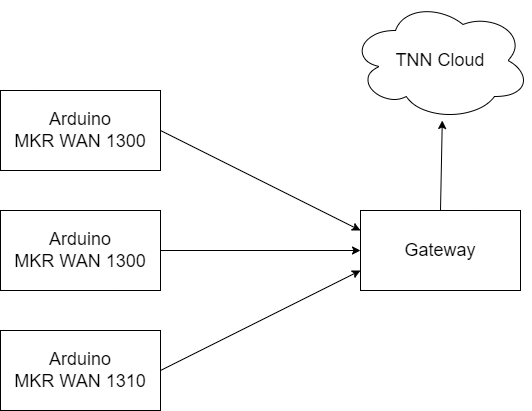
\includegraphics[scale=0.5]{Images/HW-Diagram.png}
\caption{High Level Hardware Diagram}
\label{fig:HL-HW-Diagram}
\end{figure}

The aims of this project will be satisfied once the following objectives are met.
\begin{enumerate}
\item Verify that the components selected for the IoT system are compatible and capable of transmitting and receiving data. 
\item Integrate an accelerometer into the system and write software that discretizes analog input data using the Fast Fourier Transform. 
\item Transmit the digital data from three different sensor nodes to the gateway. The gateway must be able to receive packets, identify the respective sensor node and upload the vibration payloads to the TNN cloud. 
\item Implement a solar system to constantly power the sensor nodes.
\item Design and implement a PCB carrier board for the sensor nodes.
\item Design and implement a 3D-printed enclosure to house the components of the sensor nodes. Figure \ref{fig:HL-HW-Diagram-Detailed} exhibits the detailed, high level, hardware system diagram and figure \ref{fig:HL-SW-Diagram} contains the high level, software diagram for the transmitter and receiver systems. 
\end{enumerate}

\begin{figure}[h!]
\center
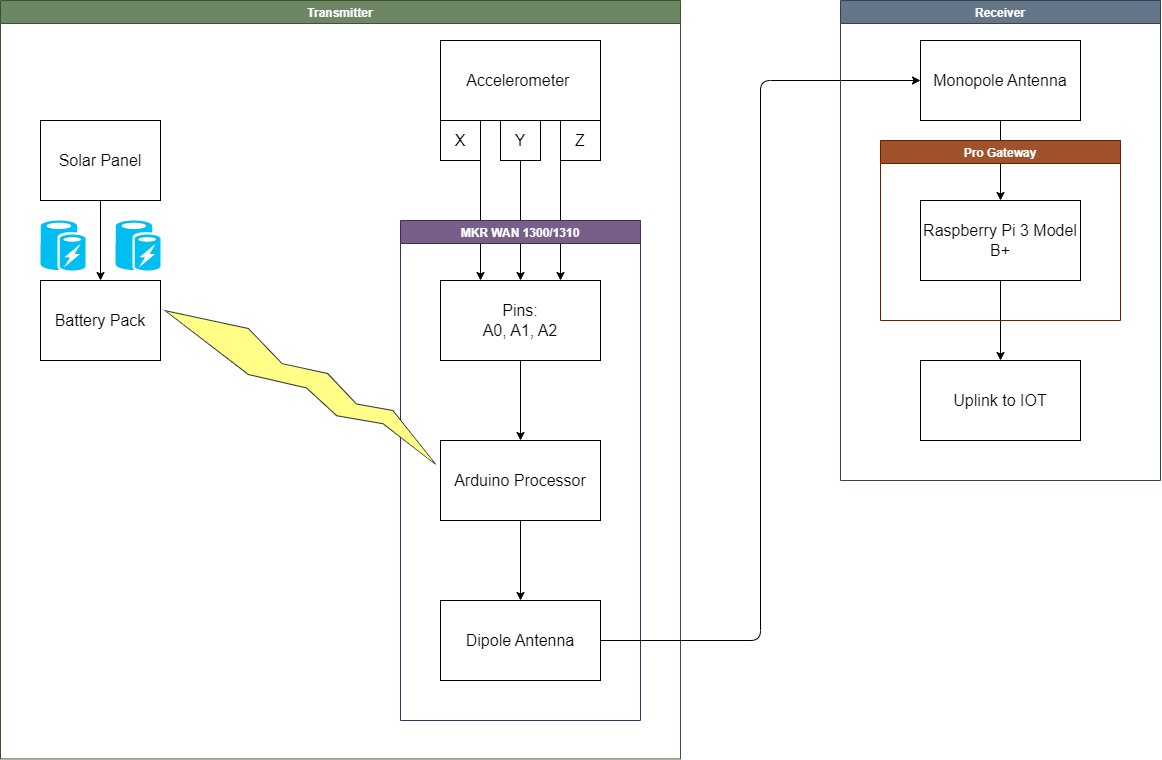
\includegraphics[scale=0.38]{Images/HW-Diagram-Detailed.png}
\caption{Detailed High Level Hardware Diagram}
\label{fig:HL-HW-Diagram-Detailed}
\end{figure}
\clearpage
\begin{figure}[h!]
\center
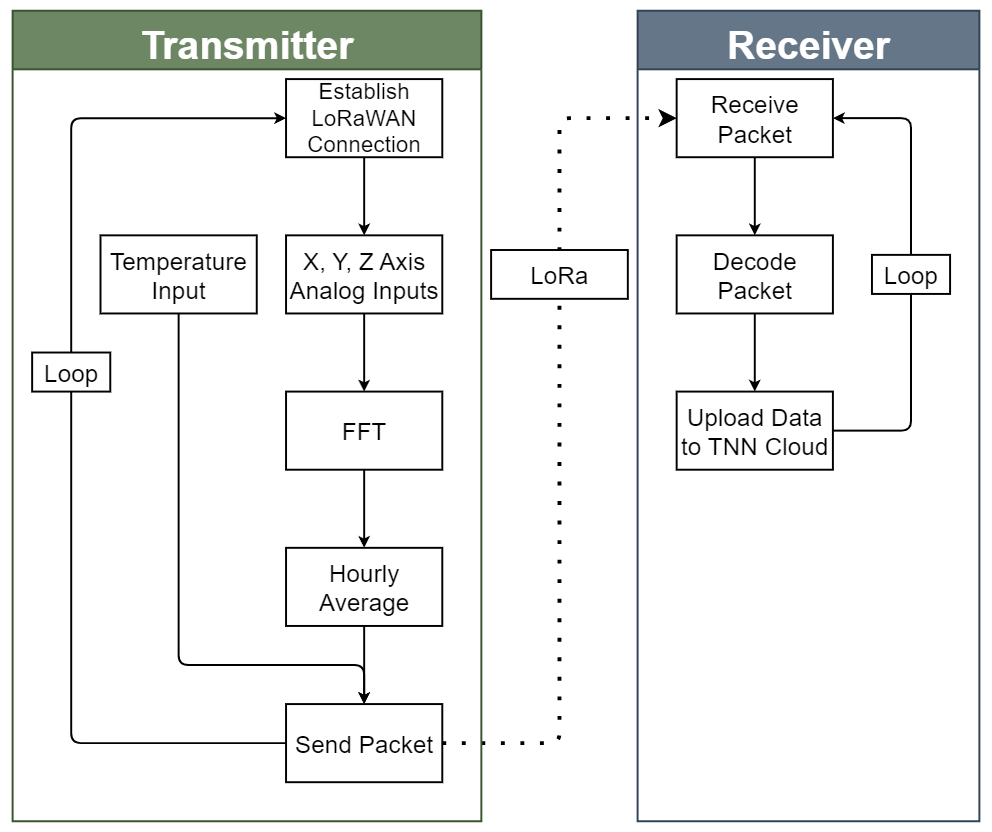
\includegraphics[scale=0.38]{Images/SW-Diagram.png}
\caption{High Level Software Diagram}
\label{fig:HL-SW-Diagram}
\end{figure}









